\imprimircapa

\imprimirfolhaderosto*

\begin{fichacatalografica}
	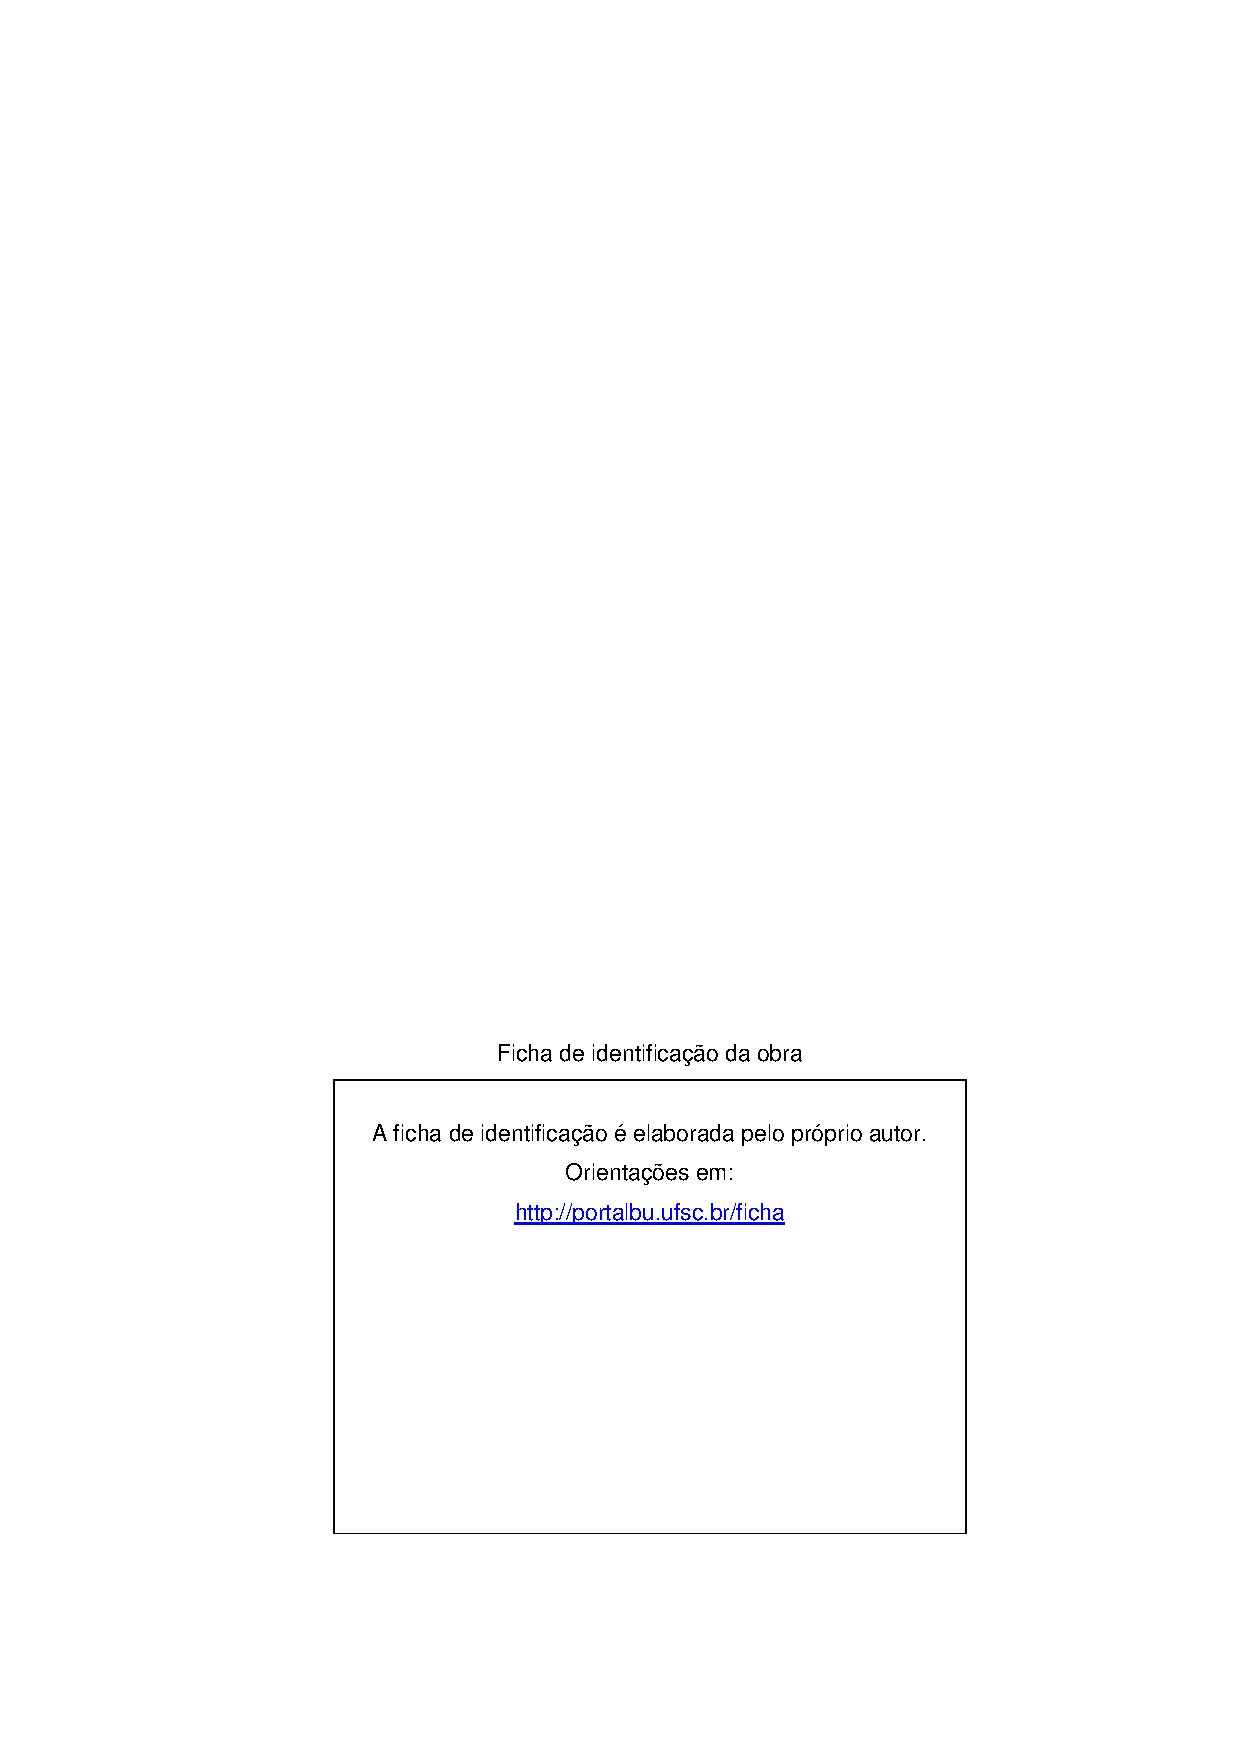
\includepdf{PreTextuais/Ficha_Catalografica.pdf}
\end{fichacatalografica}

\begin{folhadeaprovacao}
	\OnehalfSpacing
	\centering
	\imprimirautor\\%
	\vspace*{10pt}		
	\textbf{\imprimirtitulo}%
	\ifnotempty{\imprimirsubtitulo}{:~\imprimirsubtitulo}\\%
	%		\vspace*{31.5pt}%3\baselineskip
	\vspace*{\baselineskip}
	%\begin{minipage}{\textwidth}
	% ~do~\imprimirprograma~do~\imprimircentro~da~\imprimirinstituicao~para~a~obtenção~do~título~de~\imprimirformacao.
	Este~\imprimirtipotrabalho~foi julgado adequado para obtenção do Título de “\imprimirformacao” e aprovado em sua forma final pelo~\imprimirprograma. \\
		\vspace*{\baselineskip}
	\imprimirlocal, \imprimirdata. \\
	\vspace*{2\baselineskip}
	\assinatura{\OnehalfSpacing\imprimircoordenador \\ \imprimircoordenadorRotulo~do Curso}
	\vspace*{2\baselineskip}
	\textbf{Banca Examinadora:} \\
	\vspace*{\baselineskip}
	\assinatura{\OnehalfSpacing\imprimirorientador \\ \imprimirorientadorRotulo}
	%\end{minipage}%
	\vspace*{\baselineskip}
	\assinatura{Prof.(a) xxxx, Dr(a).\\
	Avaliador(a) \\
	Instituição xxxx}

	\vspace*{\baselineskip}
	\assinatura{Prof.(a) xxxx, Dr(a).\\
	Avaliador(a) \\
	Instituição xxxx}


\end{folhadeaprovacao}

\begin{dedicatoria}
    \vspace*{\fill}
    \noindent
    \begin{adjustwidth*}{}{5.5cm}     
        Aos meus pais, José Roberto dos Santos e Teresa de Jesus de Souza Aguiar, por cada sacrifício, por cada gesto de amor, por cada exemplo de dedicação. Aos meus irmãos por acreditaram em meu potencial e caminharam ao meu lado nesta jornada acadêmica. À minha namorada por ter me motivado a cada segundo do processo.
    \end{adjustwidth*}
\end{dedicatoria}

\begin{agradecimentos}
    Agradeço à Faculdade de Engenharia da Universidade Federal de Mato Grosso pela excelência acadêmica proporcionada, que enriqueceu meu conhecimento e habilidades. 
    
    Expresso minha gratidão à dedicada equipe de professores e funcionários, cujo comprometimento a frente de tantas dificuldades e complicações, não recuaram em oferecer um ensinamento completo a cada aluno, que contribuiu significativamente para o meu crescimento profissional. Esta instituição desempenhou um papel fundamental no meu desenvolvimento acadêmico, sendo um privilegiado ambiente de aprendizado.
    
    Agradeço ao professor João Gustavo Coelho Pena pela confiança, parceria, pela atenção e confiança, que possibilitou a construção desse trabalho. 
\end{agradecimentos}

\begin{epigrafe}
    \vspace*{\fill}
    \begin{flushright}
        \textit{``Não é o conhecimento, mas o ato de aprender.\\
        Não a posse, mas o ato de chegar lá\\
        Que garante o maior prazer''\\
        (Carl Friedrich Gauss)}
    \end{flushright}
\end{epigrafe}
% ---

\setlength{\absparsep}{18pt} % ajusta o espaçamento dos parágrafos do resumo
\begin{resumo}
    \SingleSpacing
    Neste trabalho de conclusão de curso, desenvolveu-se DRD (Dashboard of Data Reconciliation), um software online de análise, reconciliação e qualidade de dados utilizando técnicas de minimização de funções multivariáveis pelo método dos multiplicadores de Lagrange. A solução toma como prioridade uma abordagem baseada na web, oferecendo ao usuário a capacidade de realizar a análise e reconciliação de dados de forma remota e eficiente, com foco nos conceitos computacionais modernos afim dessa experiência ser a mais facilitada possível. Se utiliza durante todo o software a aplicação dos cálculos matemáticos e estatísticos voltados ao problema de análise, reconciliação e qualidade de dados. 
    
    Por meio da ferramenta é possível modelar todo um processo industrial e alimenta-lo com os dados oriundos da planta em questão e a partir disso analisar, reconciliar e verificar a qualidade dos dados em tempo real. O software é uma solução inovadora dado que não há um direto competidor para as funções oferecidas em um ambiente mais acessível e ágil no estado de Mato Grosso. Ao longo deste trabalho, o processo filosófico do desenvolvimento, os cálculos matemáticos, os conceitos estatísticos, computacionais e a lógica do software aplicado como solução são explicados de forma detalhada. Exemplos do código funcional e considerações finais sobre o trabalho realizado são apresentados nos últimos capítulos.
	
    \textbf{Palavras-chave}: Reconciliação de Dados. Análise de Qualidade de Dados. Desenvolvimento Web. Multiplicadores de Lagrange. Desenvolvimento de Software. Indústria 4.0.
\end{resumo}

% resumo em inglês
\begin{resumo}[Abstract]
    \SingleSpacing
    \begin{otherlanguage*}{english}
    In this undergraduate thesis, the development of DRD (Dashboard of Data Reconciliation) was undertaken, an online software for data analysis, reconciliation, and quality assessment using techniques of multivariable function minimization through the method of Lagrange multipliers. The solution prioritizes a web-based approach, providing users with the ability to remotely and efficiently perform data analysis and reconciliation, focusing on modern computational concepts to ensure a user-friendly experience. The software applies mathematical and statistical calculations throughout, specifically tailored to the problems of data analysis, reconciliation, and quality.

    Through this tool, it is possible to model an entire industrial process and feed it with data from the relevant plant, allowing real-time analysis, reconciliation, and quality verification. The software stands out as an innovative solution, as there is no direct competitor offering similar functions in a more accessible and agile environment in the state of Mato Grosso. This work details the philosophical process of development, mathematical calculations, statistical and computational concepts, and the logic of the software as an applied solution. Examples of functional code and final considerations about the work are presented in the last chapters.
    
    \textbf{Keywords}:  Data Reconciliation. Data Quality Analysis. Web Development. Lagrange Multipliers. Software Development. Industry 4.0.
    \end{otherlanguage*}
\end{resumo}

{
    \hypersetup{hidelinks}
    
    \pdfbookmark[0]{\listfigurename}{lof}
    \listoffigures*
    \cleardoublepage
    
    \pdfbookmark[0]{\listofquadrosname}{loq}
    \listofquadros*
    \cleardoublepage
    
    \pdfbookmark[0]{\listtablename}{lot}
    \listoftables*
    \cleardoublepage
        
    \imprimirlistadesiglas
    \imprimirlistadesimbolos
    
    \pdfbookmark[0]{\contentsname}{toc}
    \tableofcontents*
    \cleardoublepage
}